%%%%%%%%%%%%%%%%%%%%%%%%%%%%%%%%%%%%%%%%%%%%%%%%%%%%%%%%%%%%%

\mainmatter
\setcounter{page}{1}

\lectureseries[\course]{\course}

\auth[\lecAuth]{Lecturer: \lecAuth\\ Scribe: \scribe}
\date{October 6, 2009}

\setaddress

% the following hack starts the lecture numbering at 3
\setcounter{lecture}{2}
\setcounter{chapter}{2}

\lecture{Probability and Markov Processes}

\section{Probability of Sets}
For a $\sigma$-algebra $(\Omega, \Sigma, P)$ is the probability triple. $\Sigma$ is the $\sigma$-algebra. Then we have
\begin{itemize}
\item $A\in\Sigma \Rightarrow A^C\in\Sigma$
\item $A, B\in\Sigma \Rightarrow A\cup B\in\Sigma$
\item $A_i\in\Sigma ~\forall i\in\mathbb{N} \Rightarrow \bigcup_{i=1}^\infty A_i\in\Sigma$
\end{itemize}
Suppose $A,B\in\Sigma$, then
\begin{itemize}
\item By (a) $\Rightarrow A^C,B^C\in\Sigma$
\item By (b) $\Rightarrow A\cup B\in\Sigma$
\item By (a) $\Rightarrow (A^C\cup B^C)^C = A\cap C \therefore A\cap B\in\Sigma$
\end{itemize}
See Figure \ref{fig:03vennProb}.

\begin{figure}[ht!]
	\centering
	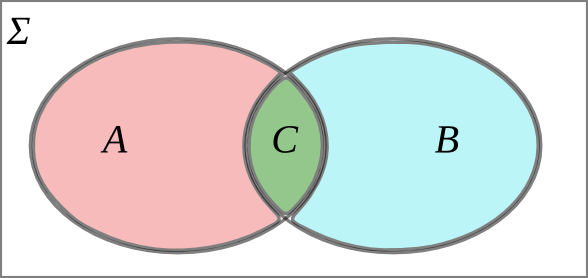
\includegraphics[width=.5\textwidth]{images/03vennProb}
	\caption{Venn diagram of the intersection of probability spaces in the set $\Sigma$.}
	\label{fig:03vennProb}
\end{figure}

\section{Conditional Probability}
Let $A,B\in\Sigma$, $P(B)>0$, then the conditional probability of $A$ given $B$ is
$$P(A|B) = \frac{P(A\cap B)}{P(B)}$$
If $A$ and $B$ are independent then
$$P(A|B) = \frac{P(A\cap B)}{P(B)} = \frac{P(A)P(B)}{P(B)} = P(A)$$
This means that if two events are independent then learning information about one of the events tells us nothing about the probability of the other event occurring.

\begin{example}
Using two tosses of a fair coin the results can be those shown in Figure \ref{fig:03coinProb}. In set $A$ we know the outcome of the first event was heads. In set B we know the outcome of the second event was heads. Knowing that we are in set $B$ tells us nothing about set $A$. In other words, knowing the outcome of the second toss tells us nothing about the outcome of the first toss. This means that the sets $A$ and $B$ are independent.
\end{example}
$\lozenge$

\begin{figure}[ht!]
	\centering
	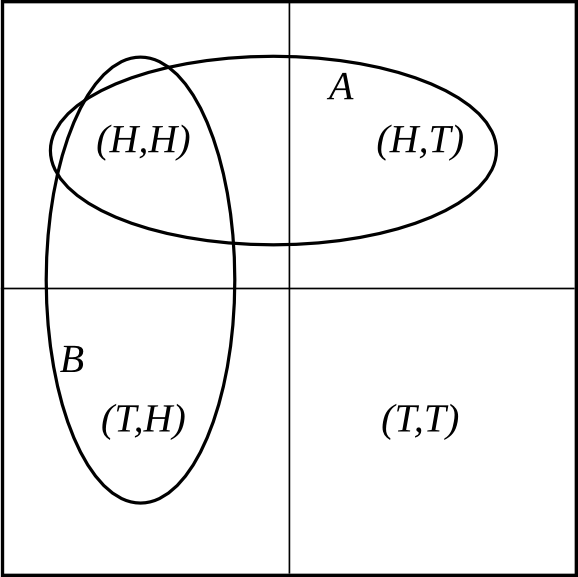
\includegraphics[width=.3\textwidth]{images/03coinProb}
	\caption{Sets representing knowledge of two fair coin tosses at different time steps.}
	\label{fig:03coinProb}
\end{figure}

\subsection{Conditioning on Sets of Probability Zero}
Suppose $X,Y$ are RVs with range $\mathbb{R}$ and joint density function $p(x,y)$. What is the density of $X$ given $Y=d$, or $P_{X|Y=d}(x)$. First, write down the distribution function for $X|Y=d$ by a limit $F_{X|Y=d}(x)$ while assuming that the density functions are continuous.
\begin{align}
\label{eq:distFn}
F_{X|Y=d}(x) &= \lim_{\delta\downarrow 0}\frac{P(X\leq x, Y\in B_\delta(d))}{P(Y\in B_\delta(d))} \\
B_\delta(d) &= \{y | |y-d| < \delta\} \nonumber
\end{align}
This gives
$$P_{X|Y=d}(x) = \lim_{\epsilon\downarrow 0}\frac{1}{\epsilon}[F_{X|Y=d}(x+\epsilon) - F_{X|Y=d}(x)]$$
which is shown in Figure \ref{fig:03probR1}.
Then, using (\ref{eq:distFn}) gives

\begin{align*}
P_{X|Y=d}(x) &= \lim_{\epsilon\downarrow 0}\frac{1}{\epsilon}\left[\lim_{\delta\downarrow 0} \frac{P(X\leq x+\epsilon, y\in B_\delta(d))}{P(Y\in B_\delta(d))} \right. \\
&\left.\quad - \lim_{\delta\downarrow 0} \frac{P(X\leq x, Y\in B_\delta(d))}{P(Y\in B_\delta(d))}\right] \\
&= \lim_{\epsilon\downarrow 0}\frac{1}{\epsilon}\left[ \frac{P(X\in(x,x+\epsilon],y\in B_\delta(d))}{P(Y\in B_\delta(d))}\right] \\
&= \lim_{\delta\downarrow 0}\lim_{\epsilon\downarrow 0}\frac{1}{\epsilon} \left[ \frac{\int_x^{x+\epsilon} \int_{d-\delta}^{d+\delta} p(z,y)dzdy}{\int_{-\infty}^\infty \int_{d-\delta}^{d+\delta} p(z,y)dzdy}\right] \\
&= \lim_{\delta\downarrow 0}\left[ \frac{\int_{d-\delta}^{d+\delta}\lim_{\epsilon\downarrow 0} \frac{1}{\epsilon} \int_x^{x+\epsilon} p(z,y)dzdy}{\int_{-\infty}^\infty \int_{d-\delta}^{d+\delta} p(z,y)dzdy}\right] \\
&= \lim_{\delta\downarrow 0} \frac{\int_{d-\delta}^{d+\delta}p(x,y)dy}{\int_{-\infty}^\infty p(z,y)dydz} \\
&= \frac{\lim_{\delta\downarrow 0}\frac{1}{2\delta}\int_{d-\delta}^{d+\delta} p(x,y)dy}{\int_{-\infty}^\infty \lim_{\delta\downarrow 0}\frac{1}{2\delta}\int_{d-\delta}^{d+\delta} p(z,y)dzdy} \\
&= \frac{p(x,d)}{\int_{-\infty}^\infty p(z,d)dz} \\
&\doteq k_dp(x,d)
\end{align*}

So, $P_{X|Y=d}(x) = k_dp(x,d)$ with $k=\frac{1}{\int_{-\infty}^\infty p(z,d)dz}$. Note that $k$ is such that $\int_{-\infty}^\infty P_{X|Y=d}(x)dx=1$. To check that do

\begin{align*}
\int_{-\infty}^\infty kp(z,d)dz &= k\int_{-\infty}^\infty p(z,d)dz \\
&= \frac{\int_{-\infty}^\infty p(z,d)dz}{\int_{-\infty}^\infty p(z,d)dz} \\
&= 1
\end{align*}

The term $p(x,d)$ is known as the ``unnormalized conditional density''. Figure \ref{fig:03deltaSpace} shows graphically the regions that are being integrated over, with those regions exagerrated for clarity.

\begin{figure}[ht!]
	\centering
	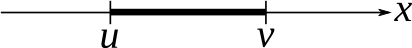
\includegraphics[width=.5\textwidth]{images/03probR1}
	\caption{Graphical depiction of the difference of probabilities at $u$ and $v$.}
	\label{fig:03probR1}
\end{figure}

\begin{figure}[ht!]
	\centering
	\includegraphics[width=.5\textwidth]{images/03deltaSpace}
	\caption{Graphical depiction of the regions being integrated over.}
	\label{fig:03deltaSpace}
\end{figure}

\section{Gaussian Distributions}
Let
$$\left(\begin{array}{c}x \\y\end{array}\right) \sim \mathcal{N}\left(\left(\begin{array}{c}0\\0\end{array}\right), C\right)$$
and
$$C^{-1} = \left[\begin{array}{c c} \rho_{xx} & \rho_{xy} \\ \rho_{xy} & \rho_{yy} \end{array}\right]$$
Also, let
\begin{align*}
\hat{k}=e^{-\frac{1}{2}\rho_{yy}d^2}, \qquad \bar{k}=\frac{1}{2\pi|C|^{1/2}},\qquad \sigma^2=\frac{1}{\rho_{xx}}, \\ m=-\frac{\rho_{xy}}{\rho_{xx}}d, \qquad \tilde{k}=\frac{1}{\sqrt{2\pi}\sigma}
\end{align*}
Then,
\begin{align*}
P_{X|Y=d}(x) &= k_dp(x,d) = k\frac{1}{2\pi|C|^{1/2}} e^{-\frac{1}{2}\left(\begin{array}{c}x\\d\end{array}\right)^TC^{-1} \left(\begin{array}{c}x\\d\end{array}\right)} \\
&= \bar{k}e^{-\frac{1}{2}\left(\rho_{xx}x^2+2\rho_{xy}xd+\rho_{yy}d^2\right)} \\
&= \hat{k}e^{-\frac{1}{2}\left(\rho_{xx}x^2+2\rho_{xy}xd\right)} \\
&= \hat{k}e^{-\frac{\rho_{xx}}{2}\left(x^2 + 2x(\frac{\rho_{xy}}{\rho_{xx}}d) + (\frac{\rho_{xy}}{\rho_{xx}})^2d^2\right)} e^{\frac{\rho_{xx}}{2}\left((\frac{\rho_{xy}}{\rho_{xx}})^2d^2\right)} \\
&= \tilde{k}e^{-\frac{\rho_{xx}}{2}\left(x+\frac{\rho_{xy}}{\rho_{xx}}d\right)^2} \\
&= \tilde{k}e^{-\frac{1}{2\sigma^2}\left(x-m\right)^2}
\end{align*}

\section{Markov Processes}
\begin{definition}{Markov Process} \\
Let $\{\xi_k\}$ be a sequence of RVs. It is a Markov process if
$$P(\xi_{t+1}\in A|\xi_r=x_r ~\forall r\leq t) = P(\xi_{t+1}\in A|\xi_t=x_t)$$
\end{definition}
The definition means that we do not have to know the history of the state to predict the future trajectory of the state.

\begin{theorem}
Let $\{w_t\}_{t=0}^\infty$ be independent and identically distributed (IID). Suppose $\xi_0$ is independent of $w_t ~\forall t$ and $\xi_{t+1} = f(\xi_t,w_t), ~\forall t \geq 0$, then $\xi_\bullet$ is Markov.
\end{theorem}

\begin{proof}
\begin{align*}
&P(\xi_{t+1}\in A | \xi_t=x_t, \xi_{t-1}=x_{t-1}, \ldots, \xi_0=x_0) \\
&\qquad = P(f(\xi_t,w_t)\in A|\xi_t=x_t, \xi_{t-1}=x_{t-1}, \ldots, \xi_0=x_0) \\
&= P(f(x_t,w_t)\in A ~|~ f(x_{t-1},w_t)=x_{t-1}, f(x_{t-2},w_{t-2})=x_{t-2},\ldots, \\
&\qquad \ldots,f(x_0,w_0)=x_1,\xi_0=x_0) \\
&\qquad [\text{let }g_x(w) \doteq f(x,w)] \\
&= P(g_{x_t}(w_t)\in A|g_{x_{t-1}}(w_{t-1})=x_t,\dots,\xi_0=x_0) \\
&= P(w_t\in(g_{x_t})^{-1}(A)|w_{t-1}\in g_{x_{t-1}}^{-1}(x_t),\ldots, w_0\in g_{x_0}^{-1}(x_1),\xi_0=x_0) \\
&= P(w_t\in g_{x_t}^{-1}(A)) ~ [\text{because of IID condition}] \\
&= P(g_{x_t}(w_t)\in A) \\
&= P(f(x_t,w_t)\in A) \\
&= P(f(\xi_t,w_t)\in A|\xi_t=x_t) \\
&= P(\xi_{t+1}\in A|\xi_t=\xi_t)
\end{align*}
\end{proof}
This proves that no history has to be stored to determine the future trajectory of the state!

\section{Linear Gaussian Case}
Let $\xi_0 \sim \mathcal{N}(m_0,C_0)$, $\{w_k\}$ be IID and $w_t \sim \mathcal{N}(m_w,C_w)$. This is known as a ``Gauss-Markov process''. Also, let the system dynamics be described by $\xi_{t+1}=A\xi_t+\sigma w_t$. Then we get
\begin{align*}
\xi_1 &= A\xi_0+\sigma w_0 \rightarrow \xi_1 \sim \mathcal{N}(m_1,C_1) \\
m_1 &= Am_0+\sigma m_w \\
C_1 &= AC_0A^T + \sigma C_w\sigma^T \\
m_2 &= Am_1 + \sigma m_w = A^2m_0 + A\sigma m_w + \sigma m_w \\
C_2 &= AC_1A^T + \sigma C_w\sigma^T = \cdots
\end{align*}

\subsection{Steady-state Distribution}
Suppose the steady-state distribution exists. Let $\bar{C} = C_n ~\forall n\geq N$, $\bar{m} = m_n ~\forall n\geq N$. Then
\begin{align*}
\bar{m} &= m_{n+1} = Am_n + \sigma m_w = A\bar{m} + \sigma m_w \\
\bar{m} &= (I-A)^{-1}\sigma m_w \\
\bar{C} &= A\bar{C}A^T + \sigma C_w\sigma^T
\end{align*}
The last equation is used to solve for $\bar{C}$.

\begin{example}
Let $w\sim\mathcal{N}(0,\rho_w^2)$, $\rho_w^2=9$, $A=\frac{1}{2}$ and $\sigma=2$. The steady-state distribution is found by $\xi_t \sim\mathcal{N}(\bar{m}, \bar{\rho}^2)$. This gives $\bar{m}=0$, $\bar{\rho}^2 = \frac{1}{2}^2(\bar{\rho})^2 + 2^2\cdot 9$.
$\lozenge$
\end{example}

\section{Optimal Controller}
Suppose the system dynamics are described by $\xi_{t+1} = f(\xi_t,u_t,w_t)$, with $\xi_t\in\mathbb{R}^n$, $u(t)\in\mathbb{R}^n$ and $w(t)\in\mathbb{R}^k$. Also, $\xi_r=x_r, ~\forall r\leq t$ are known states. Then,
\begin{align*}
&\min_{u_t\in U} E[g(t+1),\xi_{t+1}) | \xi_r=x_r ~\forall r\leq t] \\
&= \min_{u_t\in U} E[g(t+1,\xi_{t+1}) | \xi_t=x_t] \\
&= \min_{u_t\in U} E[g(t+1, f(x_t,u_t,w_t))] \\
&= \min_{u_t\in U} \int_{\mathbb{R}^n} g(t+1,f(x_t,u_t,w_t))p(w)dw \\
&= \min_{u_t\in U} G(t,x_t,u_t) \\
&\therefore \text{ optimal } u_t=\bar{u}(t,x_t) \\
&= \mu_t(x_t)
\end{align*}
This means that the optimal controller is a feedback policy.

\subsection{Control Policies}
\begin{align*}
\mathcal{M}_{\tau_1,\tau_2} &= \text{ feedbacks from } \tau_1 \text{ to } \tau_2 \\
&= \left\lbrace\left\lbrace\mu_t\right\rbrace_{t=\tau_1}^{\tau_2} | \mu_t: \mathbb{R}^n \to U, \text{ measureable } \forall t\right\rbrace
\end{align*}
If $\tau_2$ is obvious, then just write $\mathcal{M}_{\tau_1}$.

\section{Finite-time Horizon Control Problem}
The working regime is discrete-time and continuous space. The dynamics are given by
\begin{align*}
\begin{cases}
\xi_s = x, & \text{initial conditions} \\
\xi_{t+1} = f(\xi_t,u_t,w_t) & \text{else}
\end{cases}
\end{align*}
The cost-criterion or payoff, also known as the ``control policy'', is
$$J(s,x,u_\cdot) = E\left[\sum_{t=s}^{T-1} l(\xi_t,u_t) + C(\xi_t)\right]$$
where $T$ is the terminal time, $l(\cdot)$ is the running cost and $C(\xi_t)$ is the terminal cost.

The value function is
$$V(s,x) = \inf_{\mu_\bullet\in\mathcal{M}_{s,t-1}}J(s,x,\mu_\bullet)$$

%%%%%%%%%%%%%%%%%%%%%%%%%%%%%%%%%%%%%%%%%%%%%%%%%%%%%%%%%%%%%